\documentclass[11pt]{report}
\usepackage{color}
\usepackage{graphicx}
\usepackage{amsmath}
\usepackage{mathtools}
\title{\color{cyan} Analysis of Simulation \\ Sprint - 1}
\author{Amith Kumar\\and \\Sandip Baishnab}
\date{\today}

%--------------------Make usable space all of page
\setlength{\oddsidemargin}{0in}
\setlength{\evensidemargin}{0in}
\setlength{\topmargin}{0in}
\setlength{\headsep}{-.25in}
\setlength{\textwidth}{6.5in}
\setlength{\textheight}{8.5in}
%--------------------Indention
\setlength{\parindent}{1cm}

\begin{document}
%-------------------- Title Page
\maketitle
%-------------------- Contents
\tableofcontents
\newpage
\section{\color{cyan} Introduction}
An artificial agent's movement activity has been studied in this analysis. The agent will follow Markov principle to move from one place to another and generate different activity data. In reality, these data can be captured using sensors and kept in a database. We have performed simulation to analyze this movement using GAMA. GAMA comes with lot of inbuilt packages to facilitate the simulation and helps generating data from simulation for further analysis. Following sections describe about the simulation and analysis. Simulation includes  problem formulation, UML diagram of the formulated problem, Markov process , data generation and heatmap. In analytics section, basic statistics such as  variance, histograms,boxplot are discussed taking the simulated data.      

\section{\color{cyan} Simulation }
Aim of the simulation is to generate movement data (paths) across different target points, visualize and use the same data for analysis.
\subsection{Simulation Model}
1. Formation of a $50\times 50$ grid\\
2. Four targets are chosen inside the $50\times 50$ grid space\\
3. An agent would move between targets based on the markov process\\
%4. Agent always choose shortest path to reach its target\\
\subsection{UML Diagram of the Model}

\begin{figure}[h!]
  \centering
  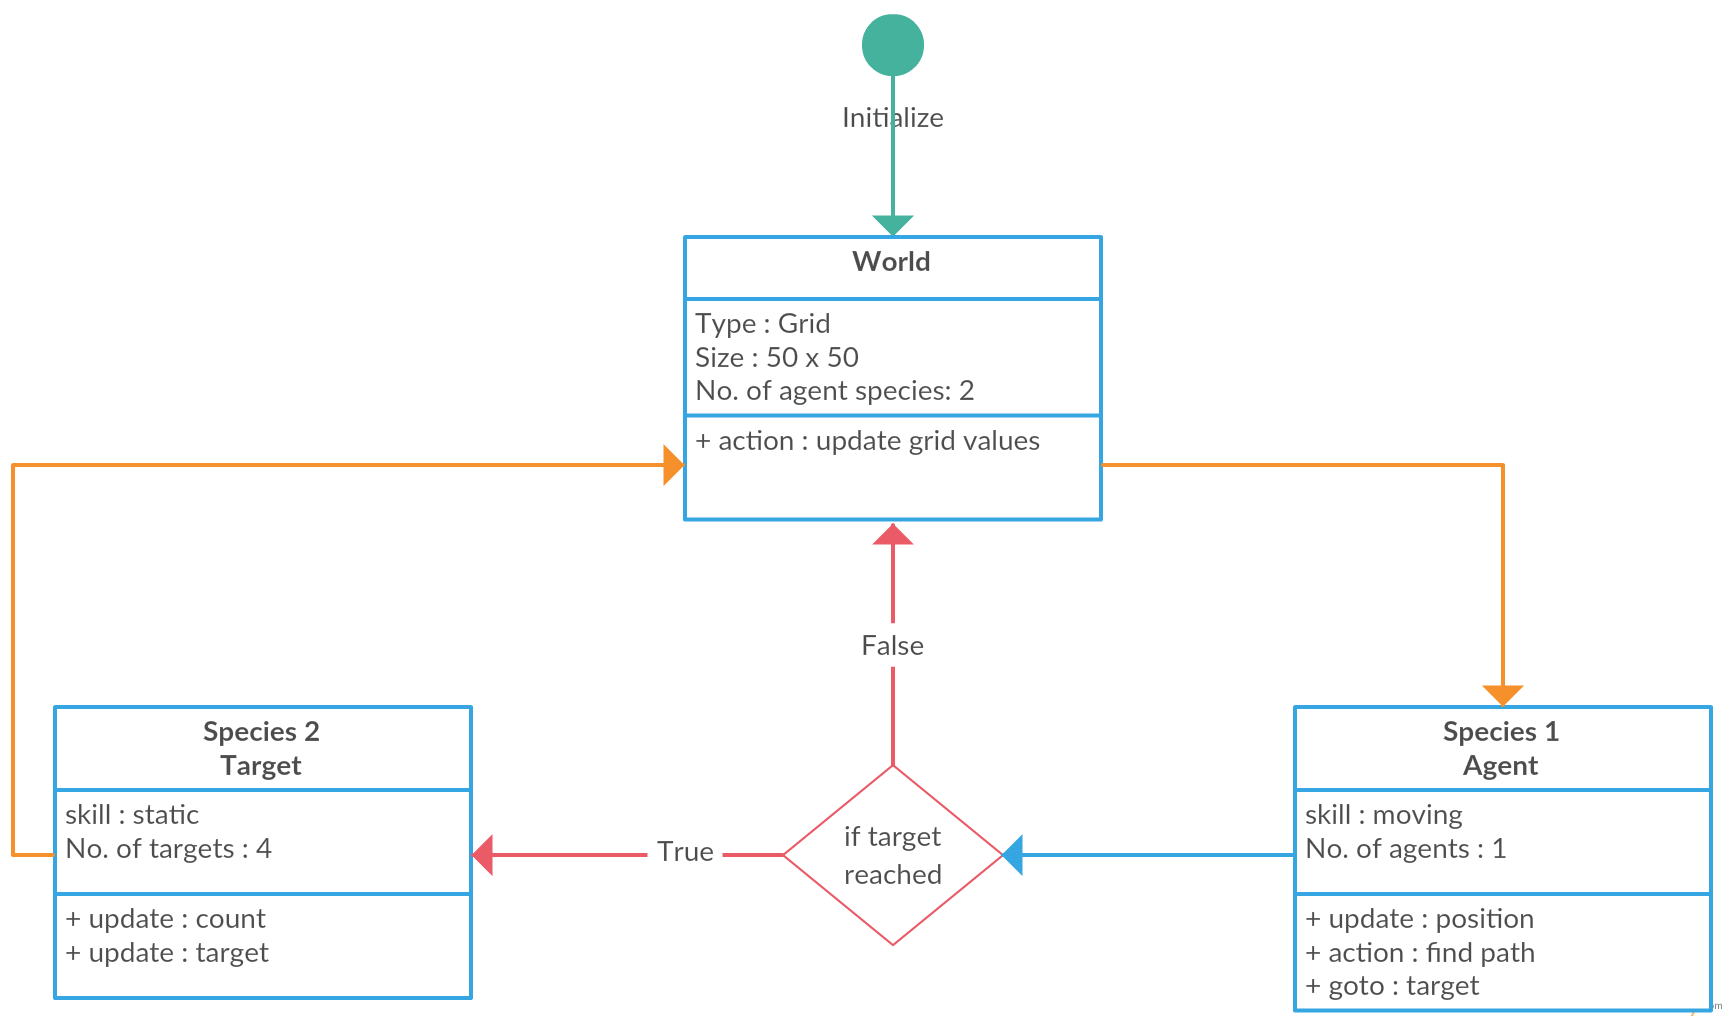
\includegraphics[height = 7cm, width = 14cm]{Simple_Grid_Move.png}
  \caption{Model}
  \label{fig:Model}
\end{figure}

\subsection{Mathematical Description of Markov Process}
Markov process is a  random process whose future probabilities are determined by its most recent values. A stochastic process $x(t)$ is called Markov if for every $n$ and $t_1<t_2...<t_n$, we have \\
\begin{center}
$ P(x(t_n)<=x_n|x(t_{n-1}),...,x(t_1)) = P(x(t_n)<=x_n|x(t_{n-1})) $.
\end{center}
This is equivalent to \\
\begin{center}
$ P(x(t_n)<=x_n|x(t) \forall t<=t_{n-1}) = P(x(t_n)<=x_n|x(t_{n-1})) $
\end{center}
 

\subsection{Data Generation for Analytics}
1. Frequency of an agent hitting the respective target points.\\
2. Frequency data from the grid to generate heatmap.\\
3. Trajectory or path information related data.
\subsection{Heatmap}

\begin{figure}[h!]
  \centering
  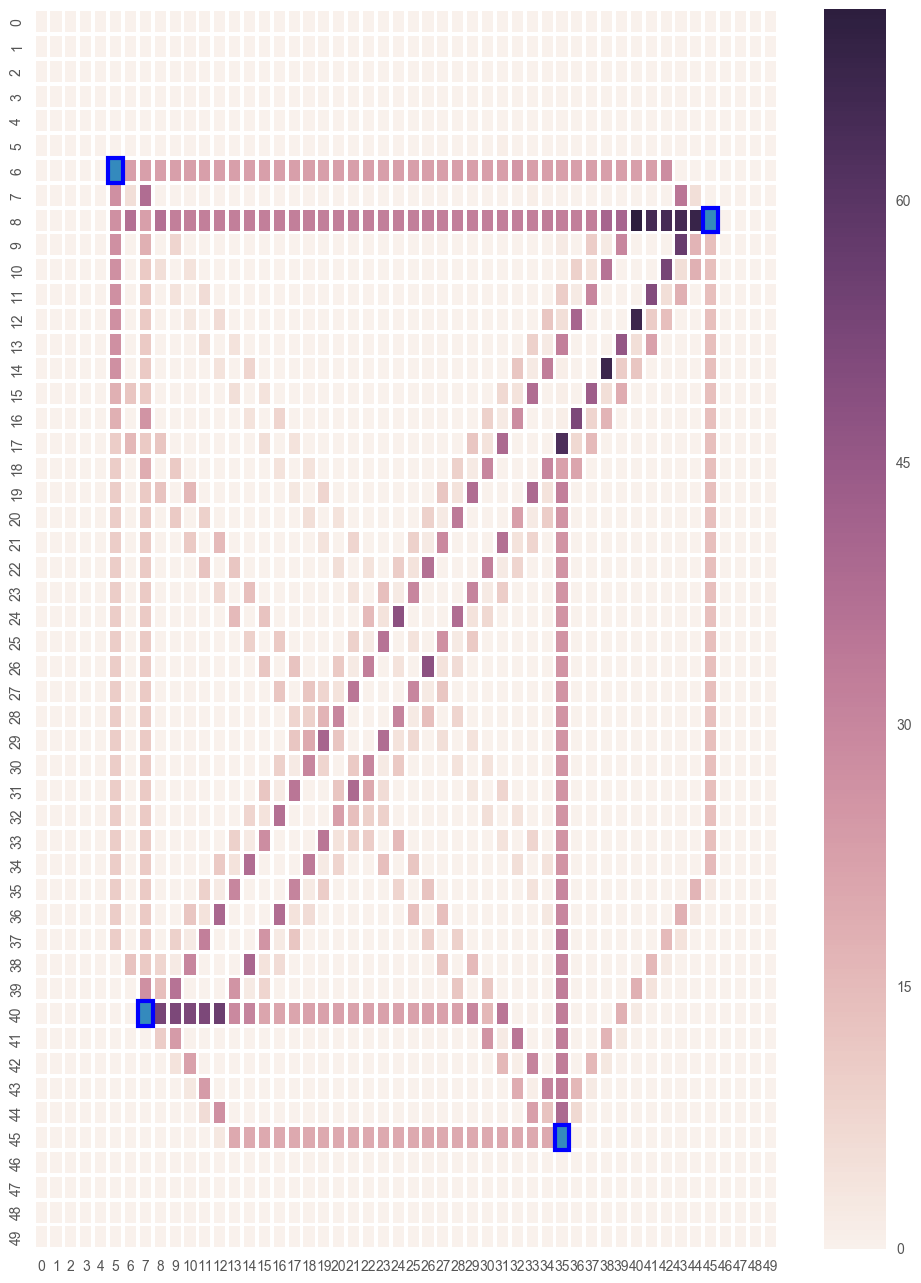
\includegraphics[height = 10cm, width = 10cm]{heatmap_2.png}
  \caption{Heatmap generated from the agent movement. Target points are represented in blue and darker color represents prominent movement of agents on respective grids.}
  \label{fig:heatmap_2}
\end{figure}


\newpage
\section{\color{cyan} Analytics}
In this part of the report, some analysis is performed on the simulated data. Following sections cover basic statistics such as total frequency, variance, histogram analysis and boxplot analysis.
For this analysis, ten times simulation are performed for generating the frequency data which describes about number of times a target is hit by an agent.

\section{Barplot}
It describes about total number of times a target has been hit during th ten simulations.

\begin{figure}[h!]
  \centering
  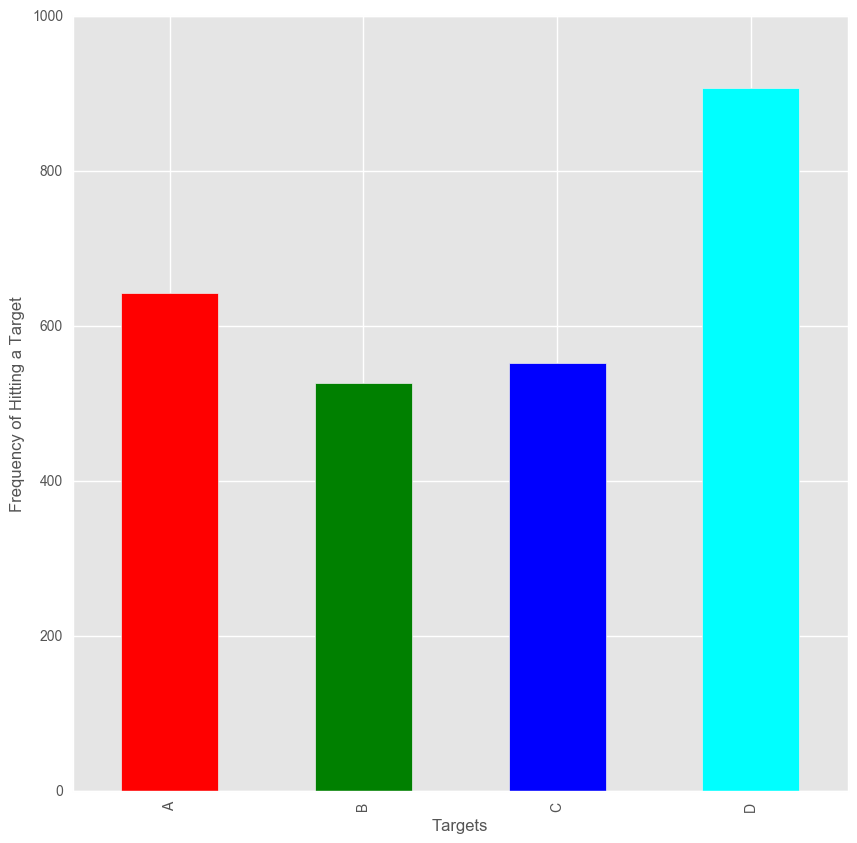
\includegraphics[height = 7cm, width = 14cm]{barplot.png}
  \caption{Barplot}
  \label{fig:barplot}
\end{figure}
\subsection{Inferences}
1. Target $D$ has been hit more than other targets during 10 simulations.\\ 
2. The plot looks like bathtub curve.

\section{Variance}
Variance has been studied to see the variance of hitting a target during 10 simulations.\\
\\
\\
\\
\\
\begin{figure}[h!]
  \centering
  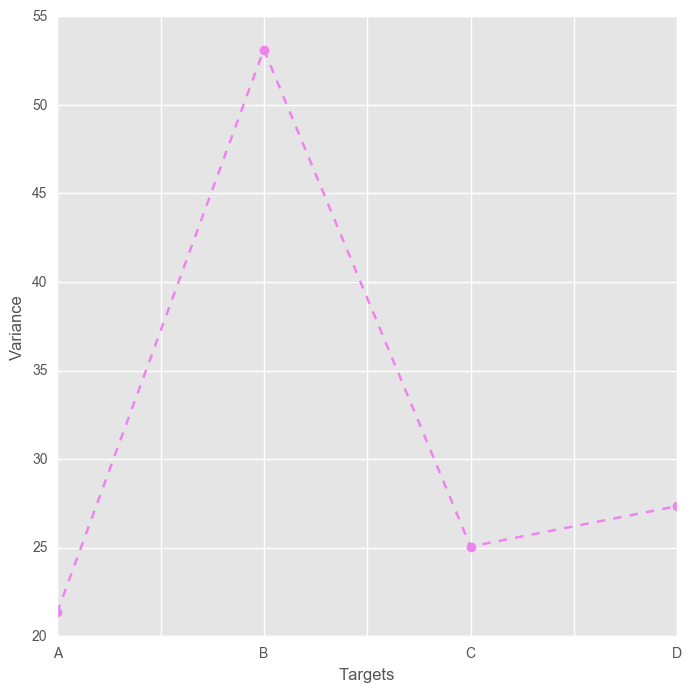
\includegraphics[height = 10cm, width = 14cm]{variance.png}
  \caption{Variance}
  \label{fig:variance}
\end{figure}

\begin{figure}[h!]
  \centering
  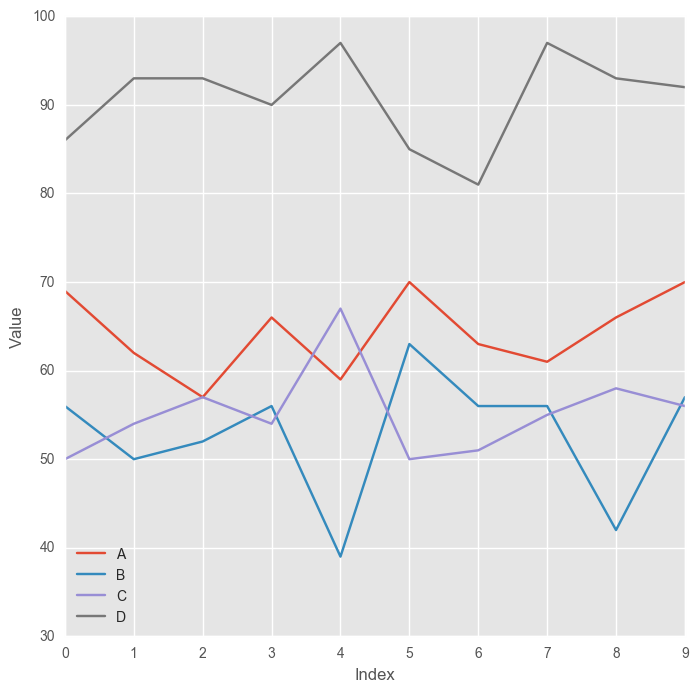
\includegraphics[height = 8cm, width = 14cm]{lineplot.png}
  \caption{Line Plot for Variance Analysis}
  \label{fig:lineplot}
\end{figure}


\subsection{Inferences}
1. Target B has highest variance \\
2. All other variances are almost same\\

\section{Hisogram}
Frequency distribution are analyzed here with bin size 4.
\subsection{Target A}
It has come out as multi-modal distribution.Frequency Values are more in the range 60-64 and 66-70.\\
\\
\\
\\
\\
\\
\\
\\
\\
\\
\\

\begin{figure}[h!]
  \centering
  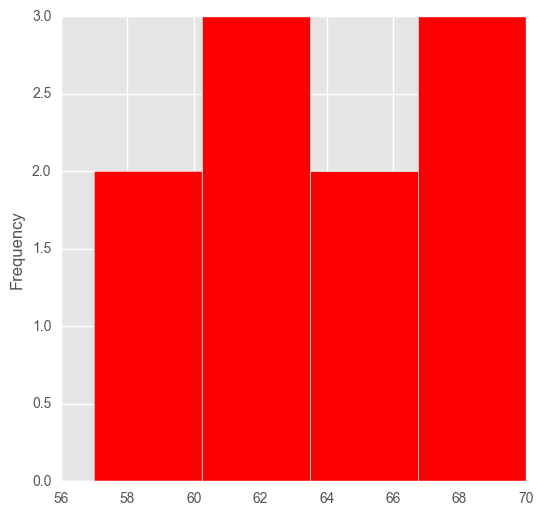
\includegraphics[height = 6cm, width = 14cm]{A_hist.png}
  \caption{Histogram of A}
  \label{fig:hist_a}
\end{figure}



\subsection{Target B}
Target $B$ is showing unimodal distribution.Frequency Values are more in the range 50-55.
\begin{figure}[h!]
  \centering
  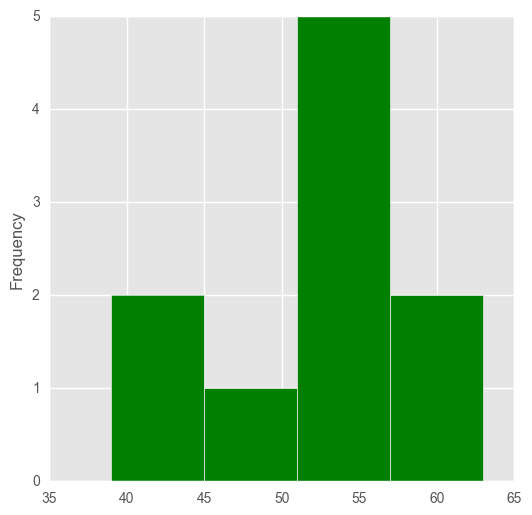
\includegraphics[height = 6cm, width = 14cm]{B_hist.png}
  \caption{Histogram of B}
  \label{fig:hist_b}
\end{figure}

\subsection{Target C}
It is almost a right skewed distribution based on the number of bins we assign to it.
\begin{center}
\begin{figure}[h!]
  \centering
  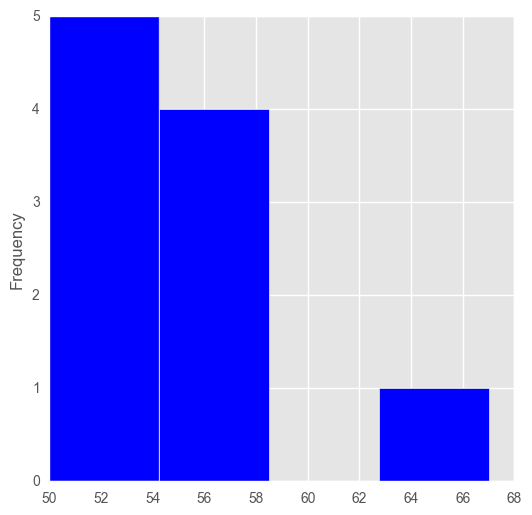
\includegraphics[height = 7
  cm, width = 14cm]{C_hist.png}
  \caption{Histogram of C}
  \label{fig:hist_c}
\end{figure} 
\end{center}

\subsection{Target D}
It is perfectly demonstrating left skewed distribution.
\begin{center}
\begin{figure}[h!]
  \centering
  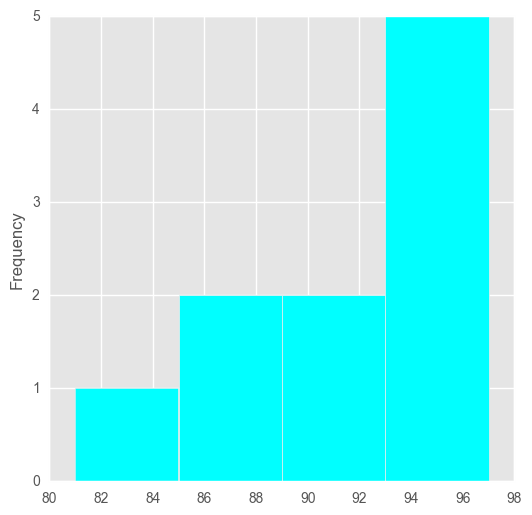
\includegraphics[height = 7cm, width = 14cm]{D_hist.png}
  \caption{Histogram of D}
  \label{fig:hist_d}
\end{figure} 
\end{center}

\section{Boxplot}
Box plot describes about minimum value, maximum value, mean, first quartile and third quartile.

\begin{figure}[!h]
  \centering
  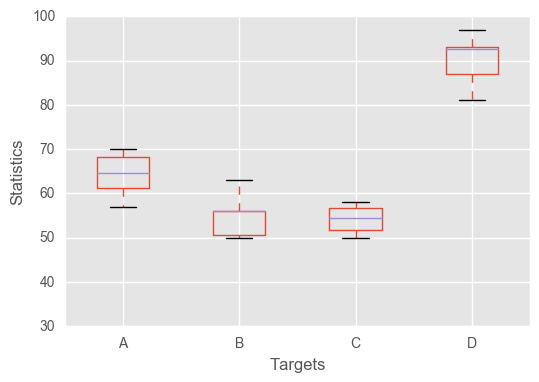
\includegraphics[height = 10cm, width = 14cm]{boxplot.png}
  \caption{Boxplot}
  \label{fig:boxplot}
\end{figure}

\subsection{Inferences}
1. For target $A$ and $C$ all statistics are distinguishable\\
2. For target $B$ and $D$ all statistics are not distinguishable\\
3. For target $B$ and $D$ median is merging with third quartile.\\

\section{Conclusion}

1. From simulation point of view, increasing the number of simulations gives better result.\\
2. Putting more targets inside the grid helps to understand  complex activity of an agent.\\
3. Multi agent environment can be studied in future.\\
4. As the simulated data comes more, analysis gets stronger with deeper insights.\\
5. Simulated trajectory data will be analyzed in future.



\end{document}